\newpage

\section{Texto Base}\label{anexo_b:texto_base}

%Artigo {\aspas{Part�culas e Intera��es} - Marco Ant�nio Moreira}.

\begin{figura}[h]
	\centering
	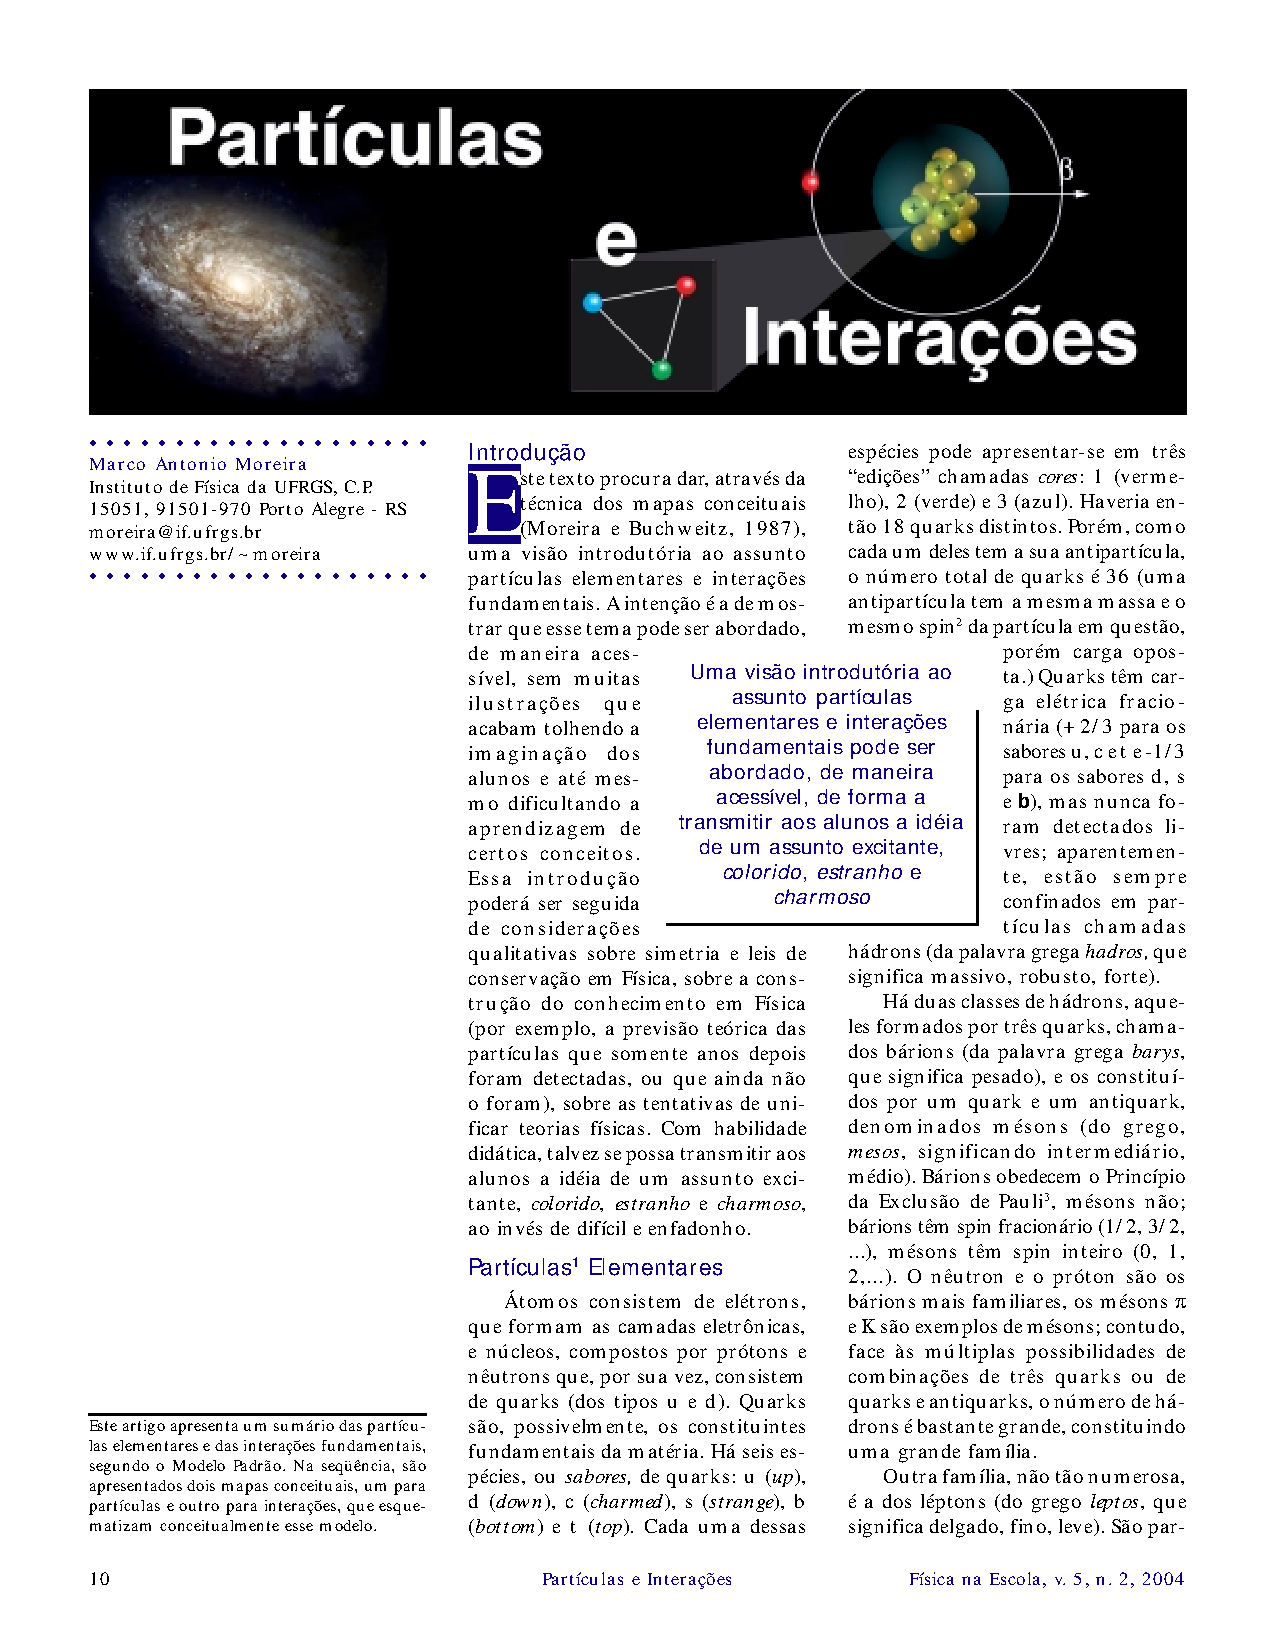
\includegraphics[width=0.89 \textwidth]{AneB/artigo_parte_1}
	\caption{Artigo: parte 1}
	\label{fig:artigo_parte_1}
\end{figura}

\newpage

\begin{figura}[h]
	\centering
	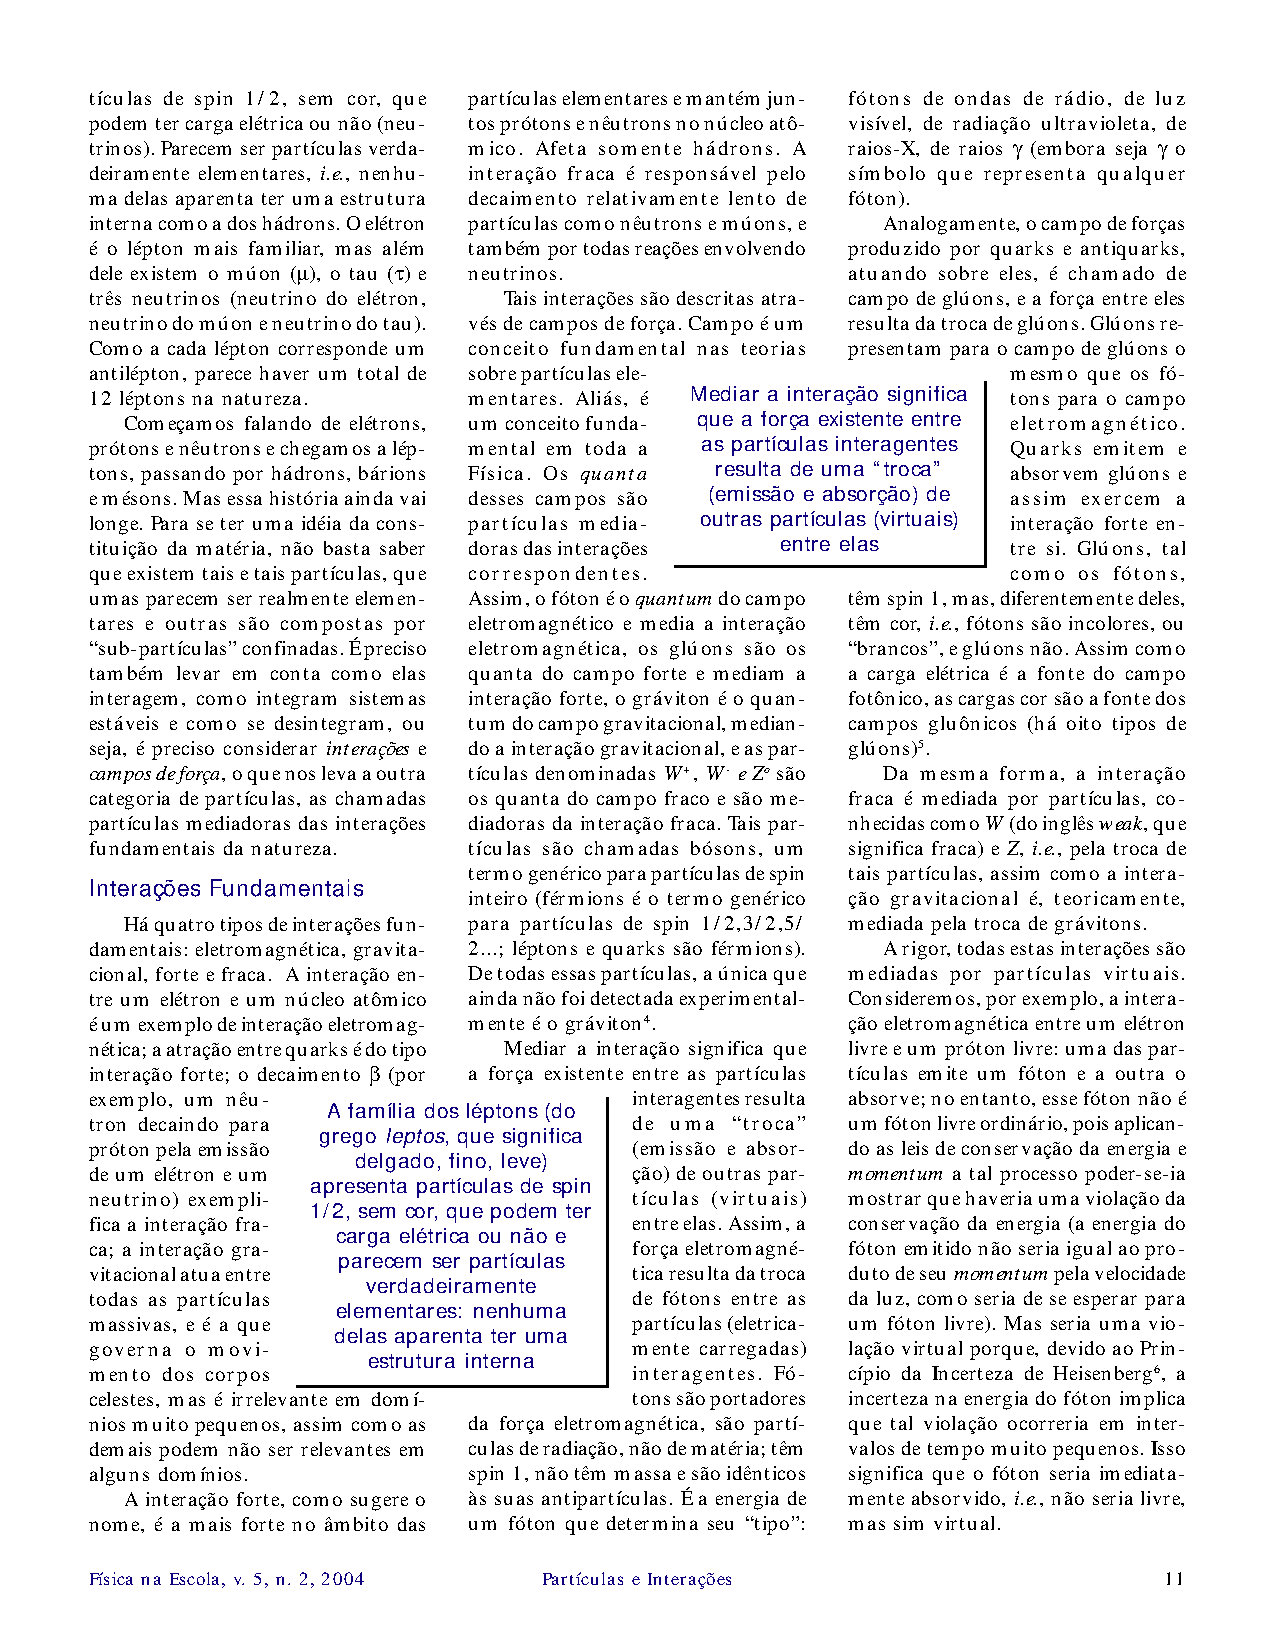
\includegraphics[width=0.89 \textwidth]{AneB/artigo_parte_2}
	\caption{Artigo: parte 2}
	\label{fig:artigo_parte_2}
\end{figura}

\newpage

\begin{figura}[h]
	\centering
	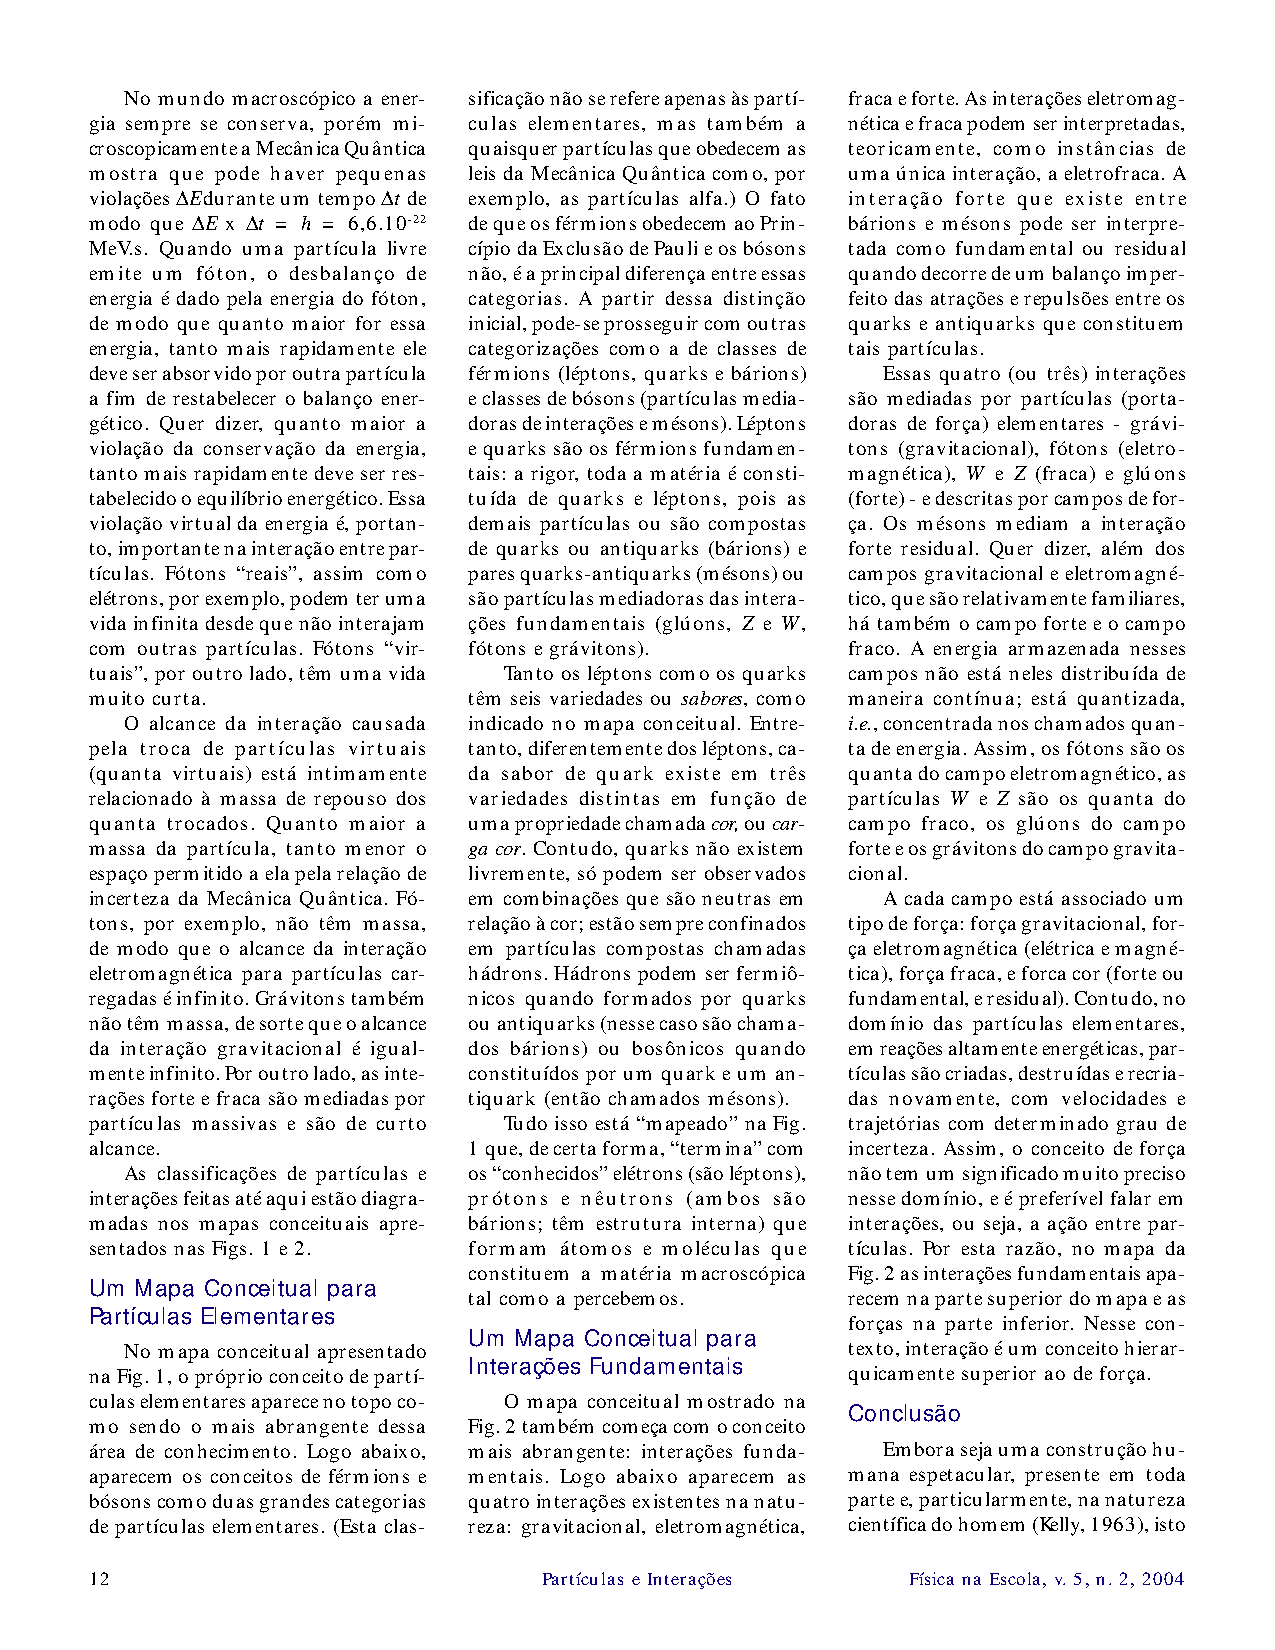
\includegraphics[width=0.89 \textwidth]{AneB/artigo_parte_3}
	\caption{Artigo: parte 3}
	\label{fig:artigo_parte_3}
\end{figura}

\newpage

\begin{figura}[h]
	\centering
	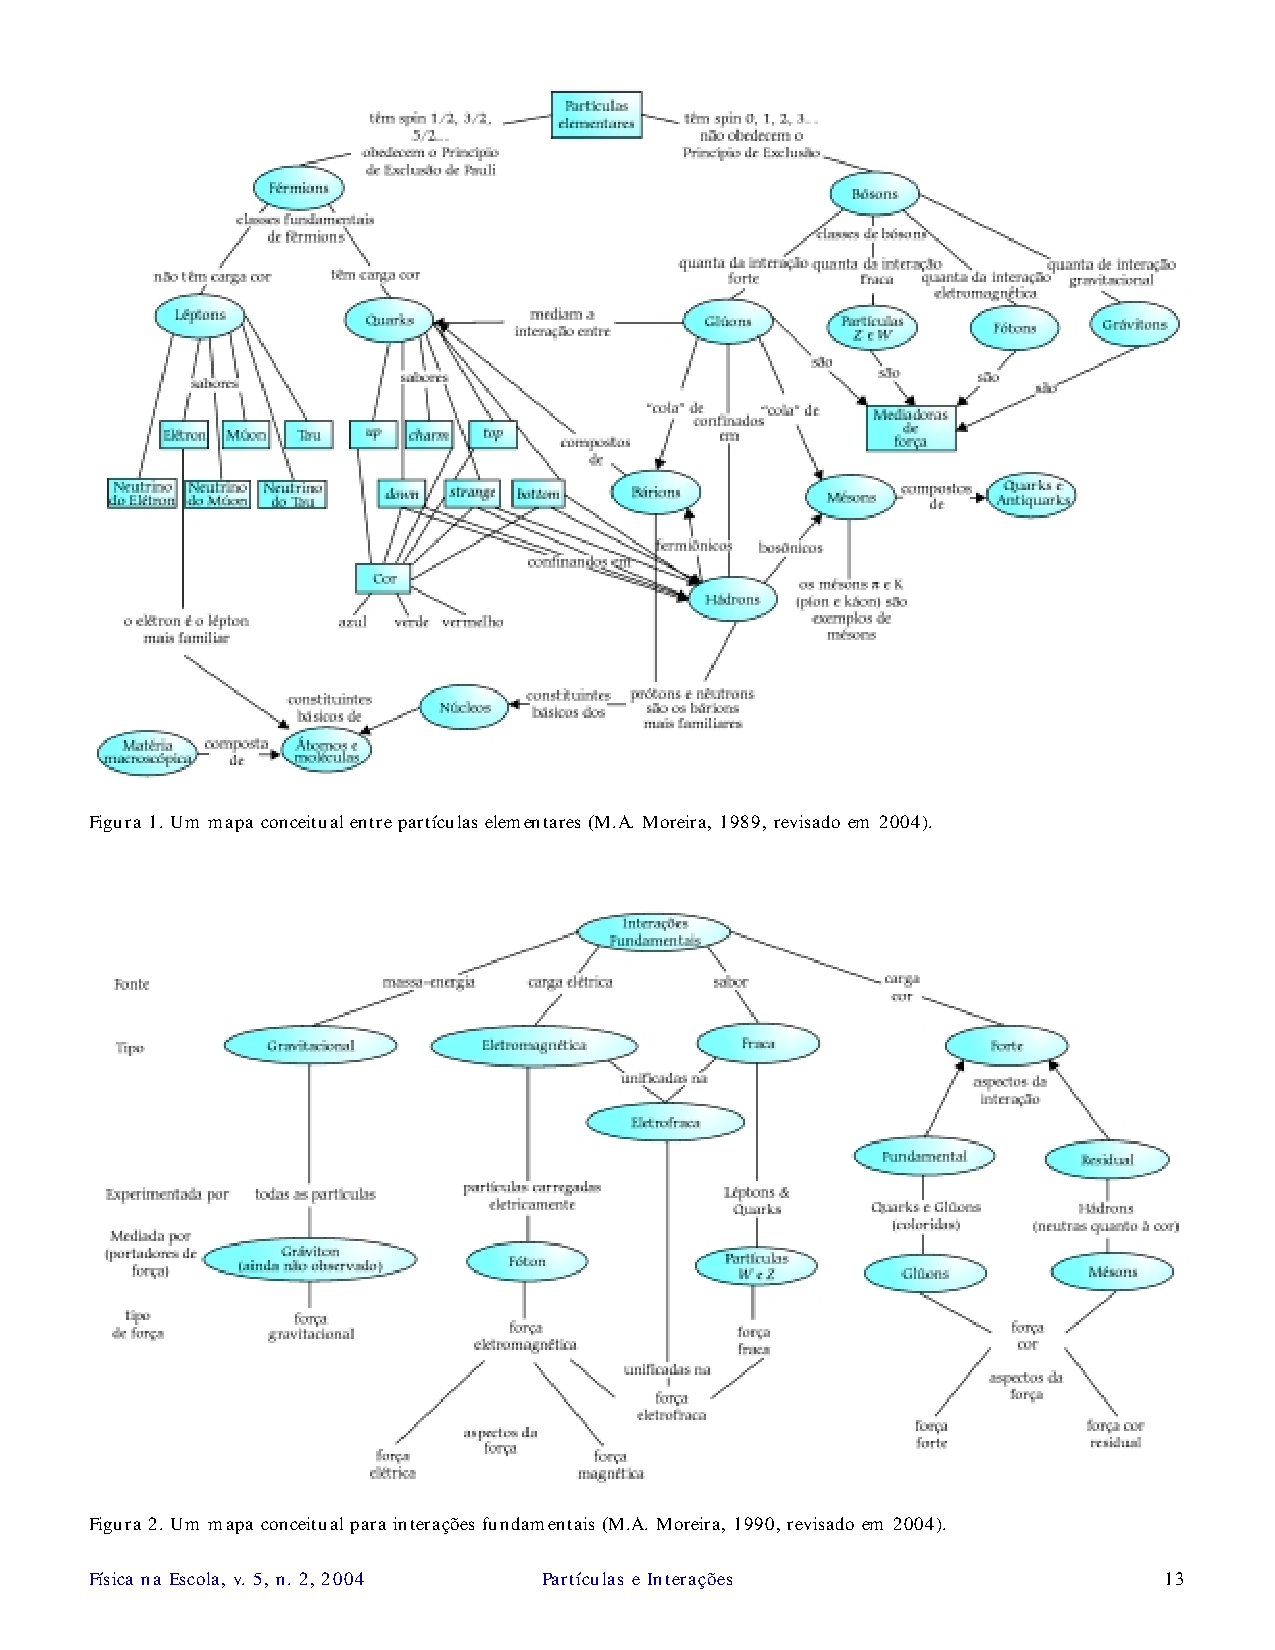
\includegraphics[width=0.89 \textwidth]{AneB/artigo_parte_4}
	\caption{Artigo: parte 4}
	\label{fig:artigo_parte_4}
\end{figura}

\newpage

\begin{figura}[h]
	\centering
	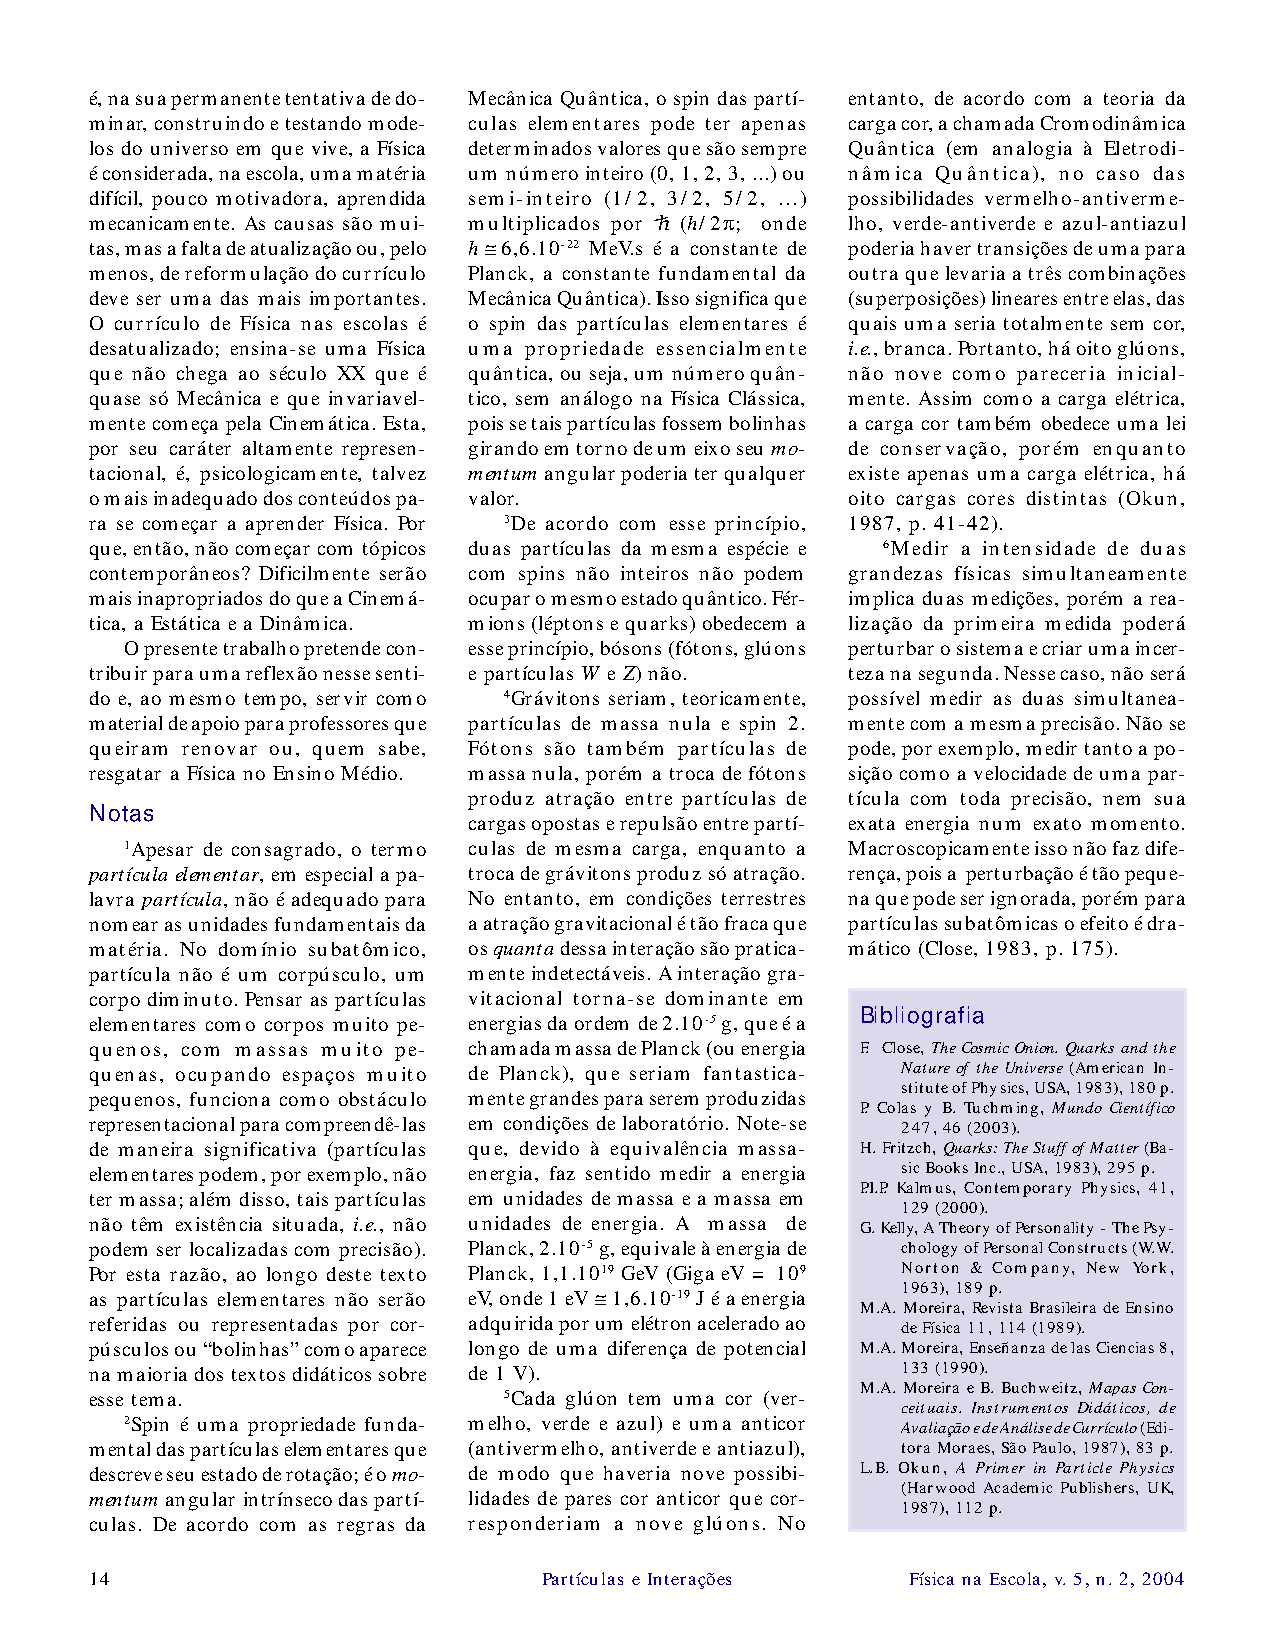
\includegraphics[width=0.89 \textwidth]{AneB/artigo_parte_5}
	\caption{Artigo: parte 5}
	\label{fig:artigo_parte_5}
\end{figura}

\newpage

\section{V�deo}\label{anexos:anexo_b:video}

\begin{figura}[h]
	\centering
	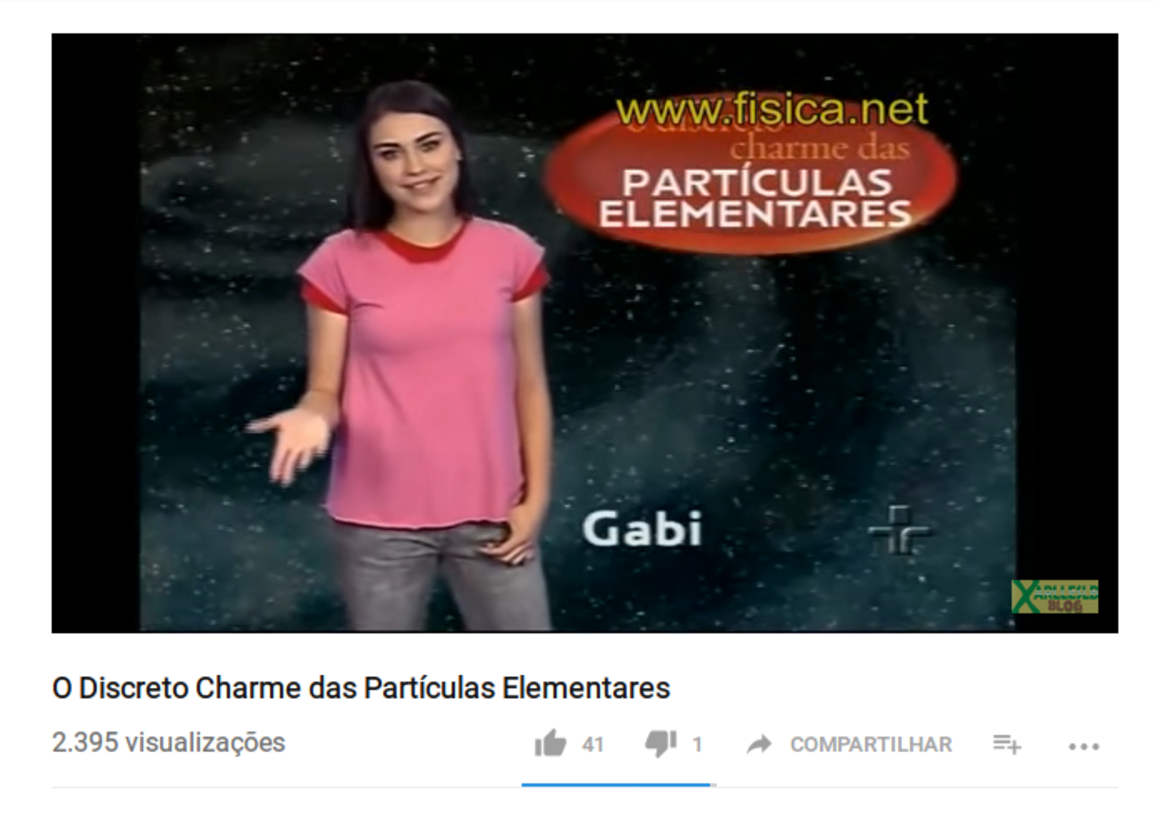
\includegraphics[width=1.0 \textwidth]{AneB/video}
	\caption{V�deo: \aspas{O Discreto Charme das Part�culas Elementares}}
	\label{anexb:fig:vid}
\end{figura}







